\documentclass{beamer}

\usepackage{color}
\usepackage{graphicx}
\usepackage{amsmath}

\newcommand{\blue}[1]{\textcolor{blue}{#1}}
\newcommand{\red}[1]{\textcolor{red}{#1}}
\newcommand {\bmu} {\mbox{\boldmath$\mu$}}

\setbeamertemplate{frametitle}[default][center]

\begin{document}

\begin{frame}
\begin{center}
\blue{\Large\bf Triggering Neoclassical Tearing Modes in NSTX}\\[2ex]
Richard Fitzpatrick\\[0.5ex]
Institute of Fusion Studies, University of Texas at Austin
\end{center}


\end{frame}

\begin{frame}
\frametitle{Motivation}
 
\begin{itemize}
\item Well-known that potentially unstable neoclassical tearing modes (NTMs) in tokamak plasmas are \red{meta-stable}.\footnote{R. Fitzpatrick, 
Phys.\ Plasmas {\bf 2}, 825 (1995).}
\item In other words, such NTMs require some sort of externally applied ``kick'' before they can grow and saturate at large amplitudes.
\item What can provide this kick? 
\item Generally assumed that kick is \red{transient magnetic perturbation} due to other modes that occur in plasma: e.g., sawtooth crashes, edge localized modes, other NTMs, etc.
\item However, there has been very little systematic investigation into what properties a transient magnetic
perturbation needs to possess in order to successfully trigger NTMs. 
\item Present talk is first step in such an investigation. 
\end{itemize}
\end{frame}

\begin{frame}
\frametitle{NSTX Shot 127317}
\frametitle{EPEC Code}
 
\begin{itemize}
\item EPEC code\footnote{R. Fitzpatrick, S.K.~Kim, and J.~Lee, Phys.\ Plasmas {\bf 28}, 082511 (2021).} simulates tearing mode dynamics in tokamak plasma using an \red{asymptotic matching} approach. 
\item Code incorporates magnetic equilibrium data (g-file) and profile data (p-file). 
\item Code includes toroidal coupling between different tearing modes. 
\item Code incorporates accurate neoclassical model that includes impurities\footnote{S.P.~Hirshman and D.J.~Sigmar, Nucl.\ Fusion {\bf 21}, 1079 (1981).} and allows calculation of bootstrap
drive to tearing modes. 
\item For case of NSTX, external perturbation is provided by pulsing RMP coils. However, perturbation is allowed to rotate.
This mimics multi-harmonic rotating magnetic perturbation generated by sawtooth crash, etc.
\end{itemize}
\end{frame}

\begin{frame}
\frametitle{NSTX Shot 127317}
 
\begin{itemize}
\item NSTX shot 127317 was used in the ELM destabilization via externally applied non-axisymmetric
resonant magnetic perturbation (RMP) experiments on NSTX.\footnote{J.M.~Canik, et al.\ Nucl.\ Fusion {\bf 50}, 034012 (2010).}
\end{itemize}
\end{frame}

\begin{frame}
\frametitle{NSTX Shot 127317: Magnetic Flux-Surfaces}

\begin{center}
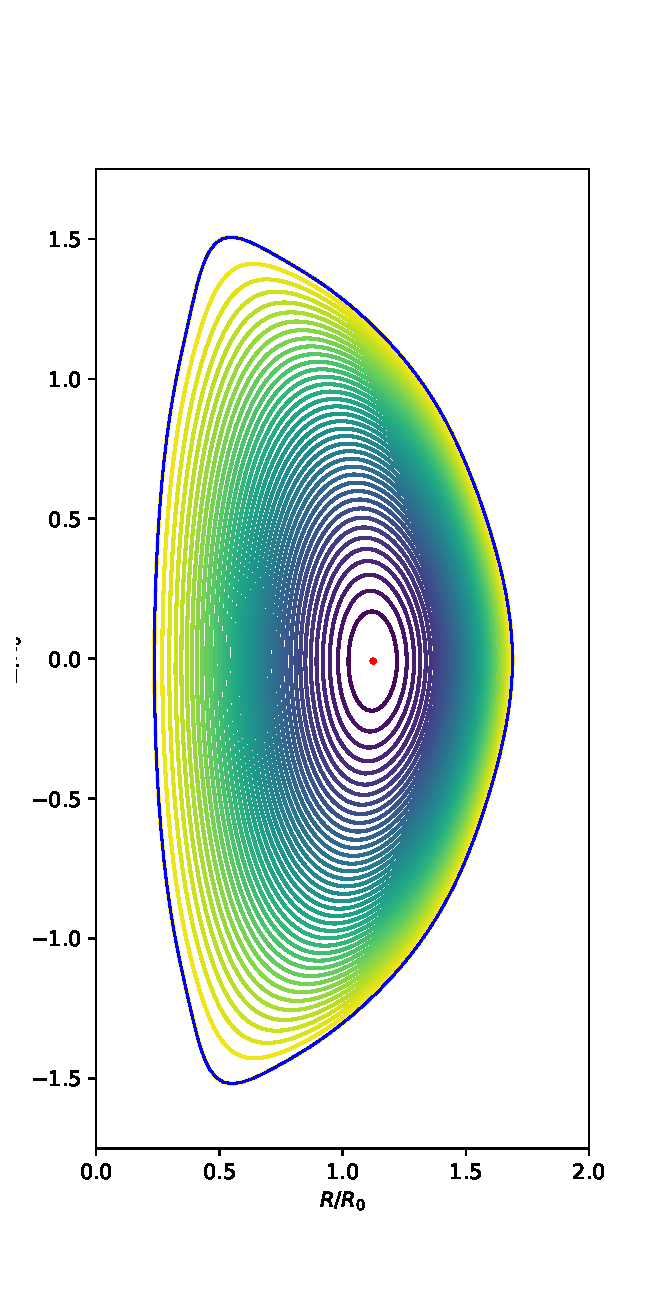
\includegraphics[height=3.6in]{Equilibrium.eps}
\end{center}

\end{frame}

\begin{frame}
\frametitle{NSTX Shot 127317: Profiles}

\begin{center}
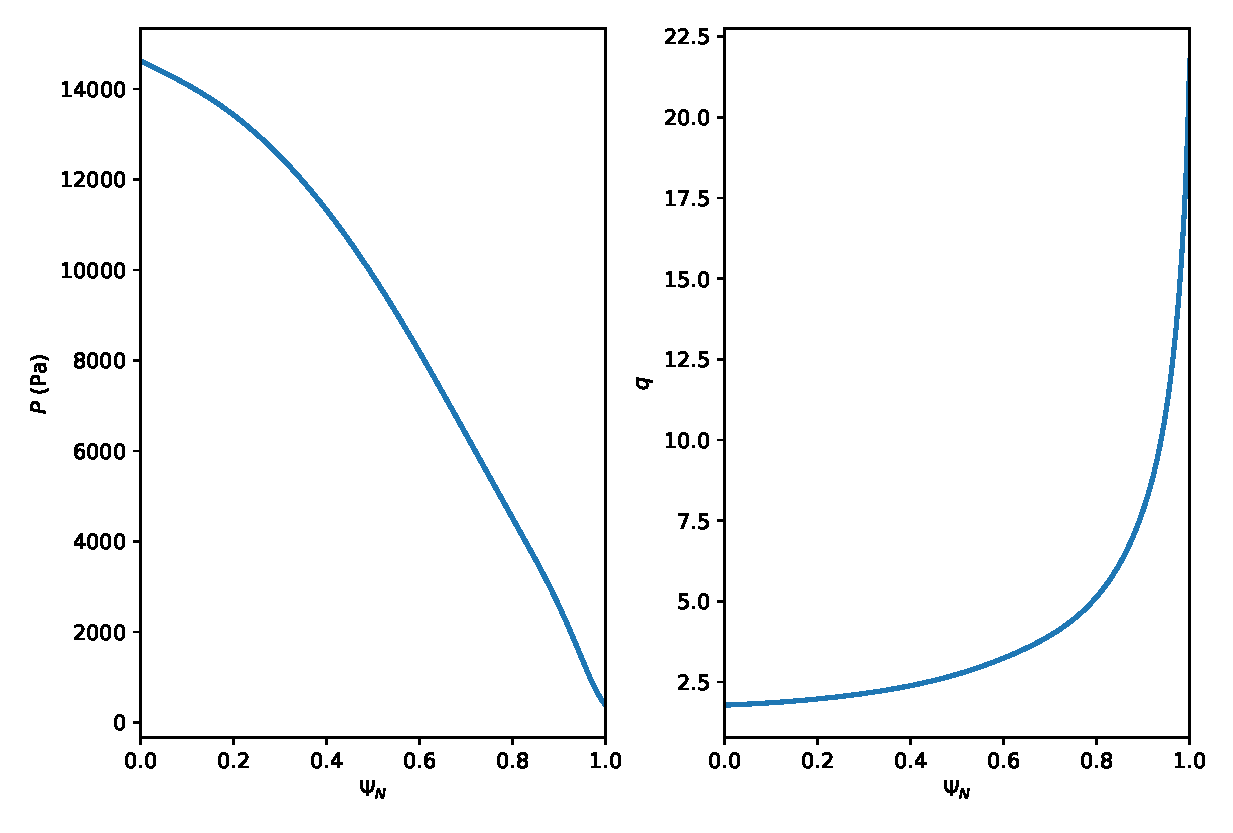
\includegraphics[width=\textwidth]{Profiles.eps}
\end{center}

\end{frame}

\begin{frame}
\frametitle{NSTX Shot 127317: $n=1$ Natural Frequencies}

\begin{center}
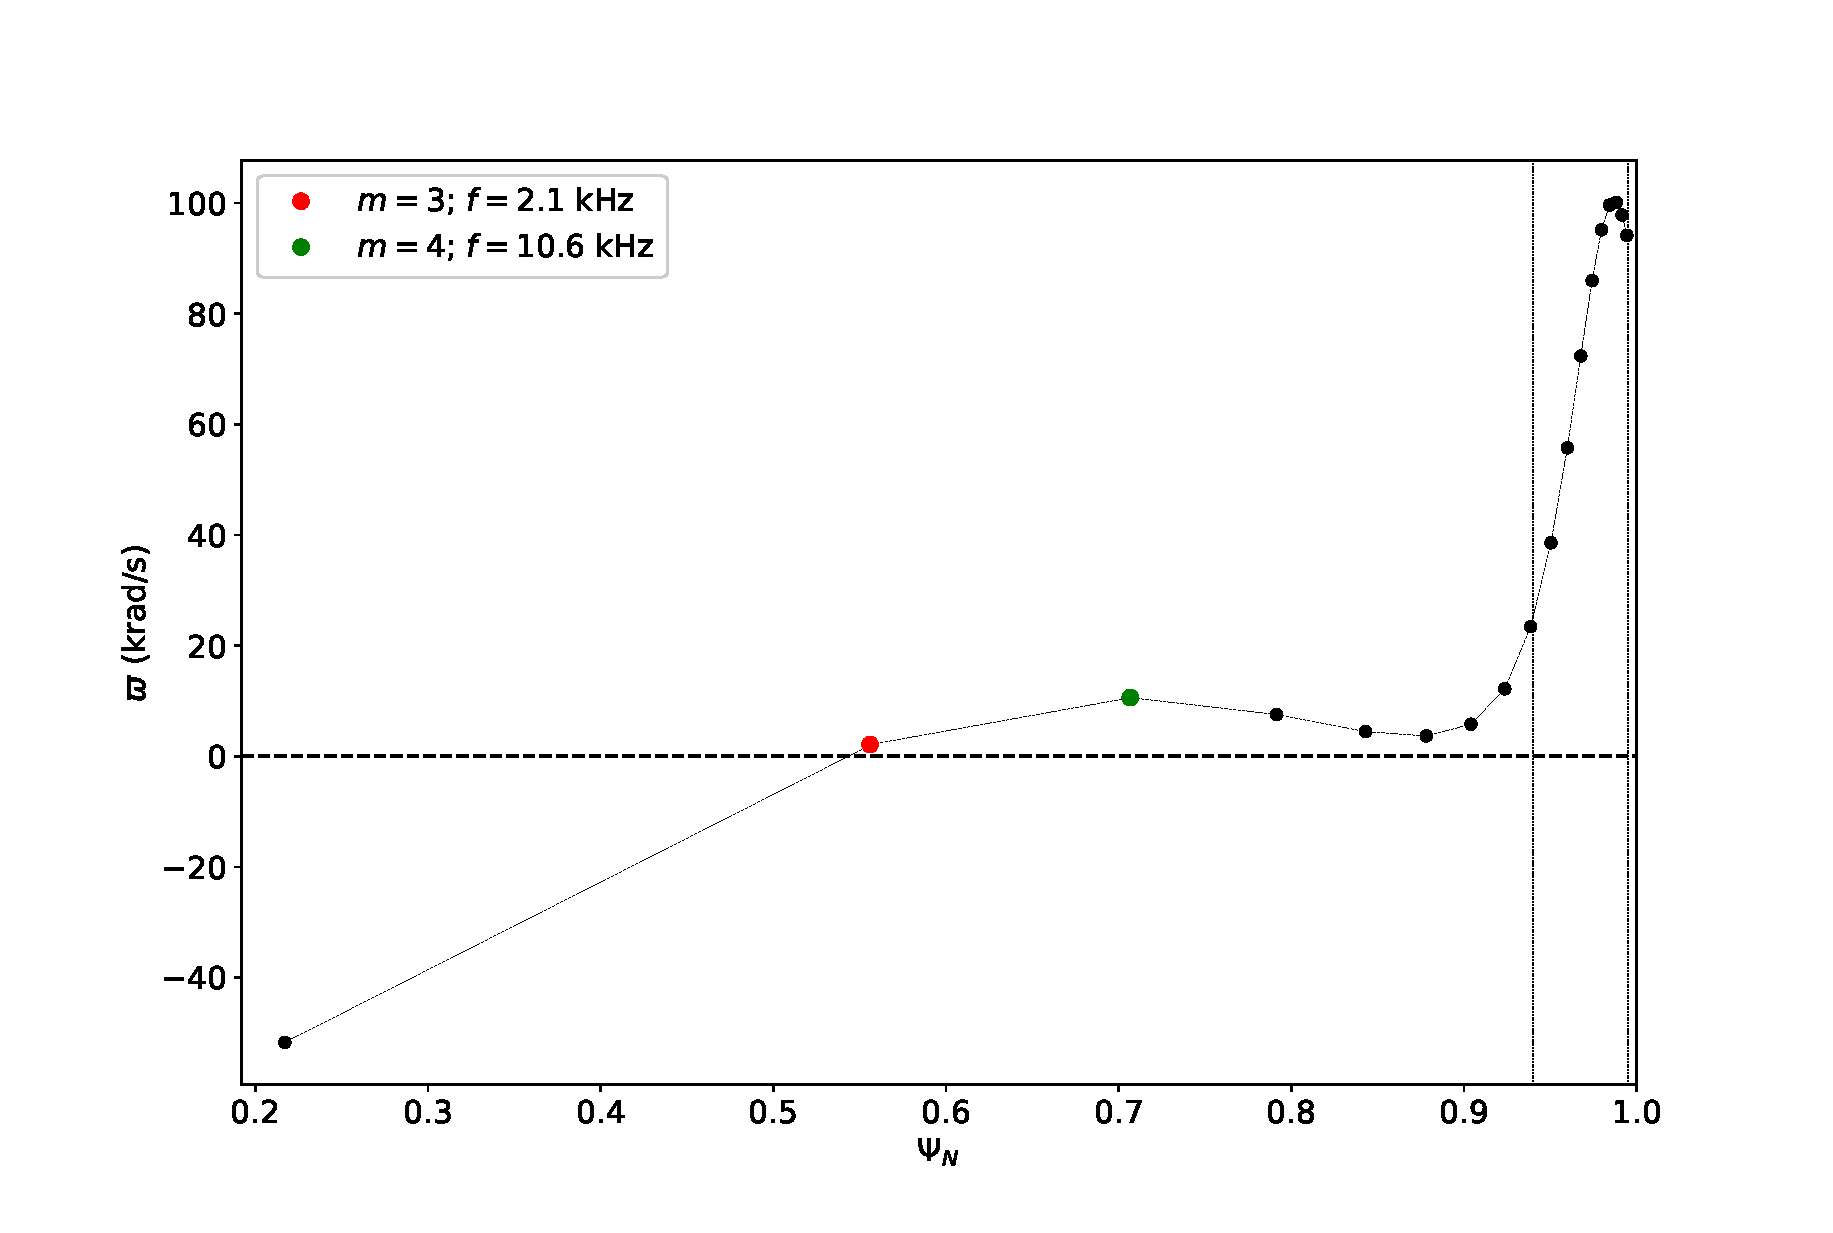
\includegraphics[width=\textwidth]{Frequency.eps}
\end{center}
\end{frame}

\begin{frame}
\frametitle{NSTX Shot 127317: $n=1$ Modes}
\begin{itemize}
\item NSTX shot 127137 (400 ms) contains \blue{18 $n=1$} rational surfaces, corresponding to \blue{$m=2$} through
\blue{$m=19$}. 
\item Only two of these surfaces, {$m=3$} and \blue{$m=4$}, are potentially unstable to NTMs.  
\item The \red{natural frequencies} (i.e., frequencies that modes would rotate at if they were naturally unstable) of
these modes are \blue{2.1 kHz} and 10.6 kHz, respectively. 
\item Natural frequencies determined by \blue{${\bf E}\times {\bf B}$} flows, diamagnetic effects, and neoclassical
effects. 
\item EPEC determines natural frequencies from experimental profile data (p-file). However, since there is no
poloidal rotation data in NSTX, poloidal rotation is given its neoclassical value (including impurities and neutrals). 
\end{itemize}
\end{frame}

\begin{frame}
\frametitle{NSTX Shot 127317: Rutherford Island Equation Rhs}

\begin{center}
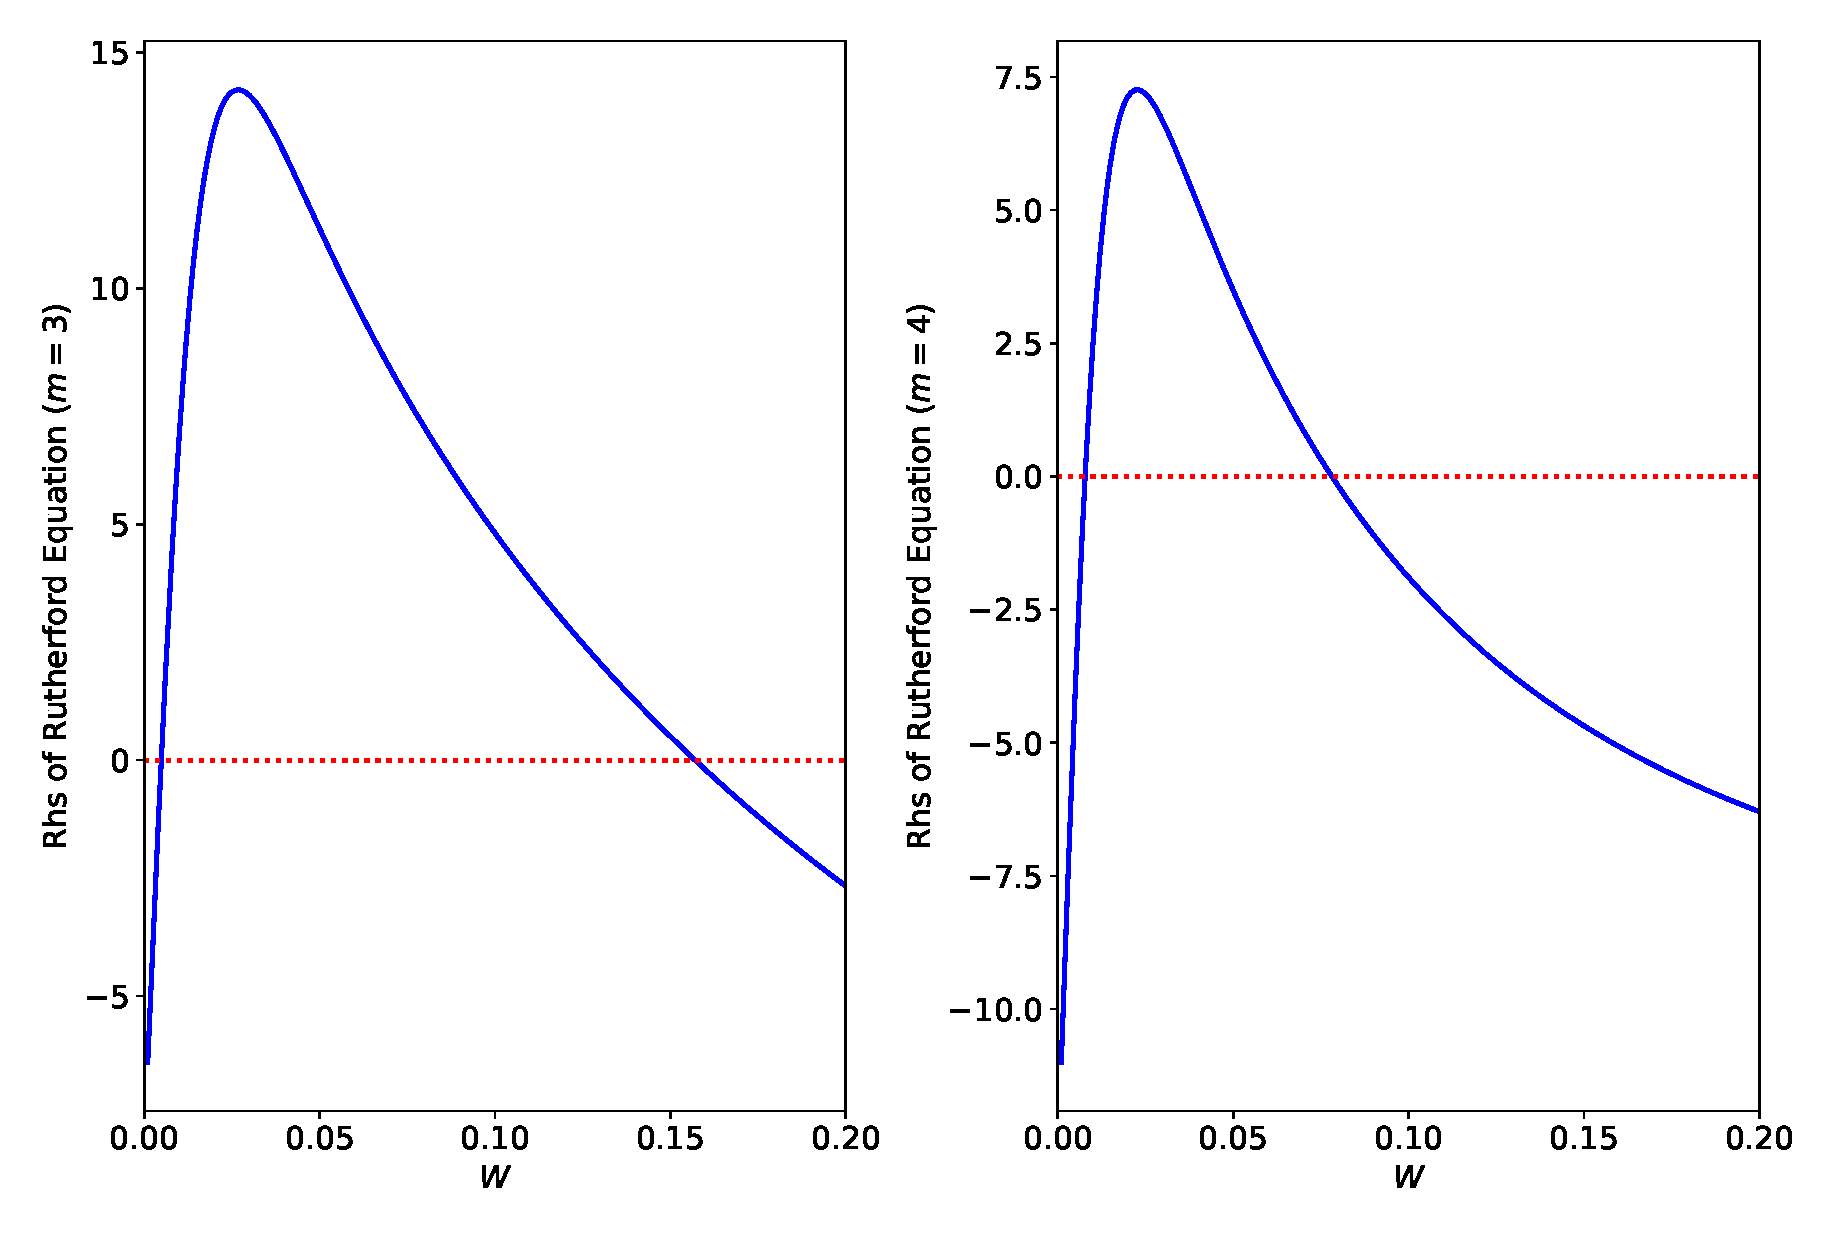
\includegraphics[width=\textwidth]{Rhs.eps}
\end{center}
\end{frame}

\begin{frame}
\frametitle{NSTX Shot 127317: Neoclassical Tearing Modes}

\begin{itemize}
\item Previous figure shows that \blue{$m=3$} and \blue{$m=4$} modes are meta-stable NTMs.
\item Both modes have potential to grow to large amplitudes (\blue{$W/a\sim 0.16$} and \blue{$W/a\sim 0.08$},
respectively). 
\item No other \blue{$n=1$} modes in plasma have Rutherford equation right-hand sides that rise above zero (i.e.,
they are all intrinsically stable).
\end{itemize}
\end{frame}

\begin{frame}
\frametitle{NSTX Shot 127317: External Peturbation}
\begin{itemize}
\item According to EPEC, if \blue{$n=1$} simulation started in initial state in which all modes have very small
amplitudes then mode amplitudes remain very small indefinitely. In other words, unperturbed plasma is
stable.
\item Apply external magnetic perturbation to system by applying square-wave \blue{$n=1$} current pulse to RMP coils. 
\item Pulse has three properties:
\begin{itemize}
\item Amplitude - kA.
\item Temporal extent (period)  - ms.
\item Phase velocity - krad/s.
\end{itemize}
\item How do these properties affect ability of pulse to trigger NTMs?
\end{itemize}

\end{frame}


\end{document}